\begin{figure}
\centering
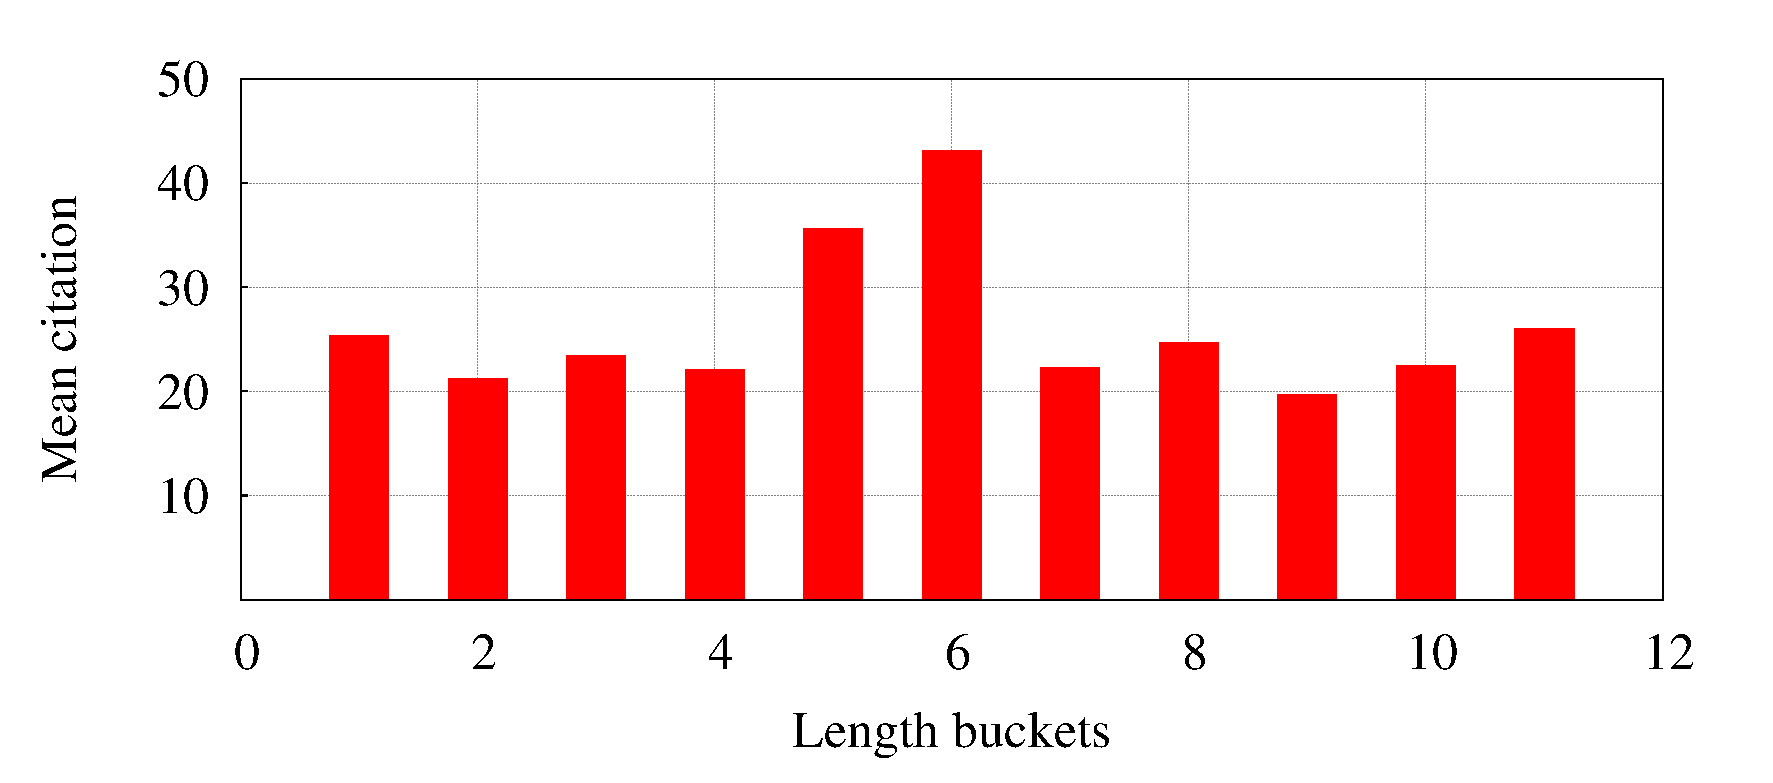
\includegraphics[scale=0.25]{./texfiles/Chapter_4/jcdl/figures/len_citation.eps}
\caption{Mean length of referee reports in terms of number of words at different rounds of review. Typically the buckets are $< 100$, ($\geq 100, < 200$) and so on}
\label{fig:length}
\vspace{3mm}
\end{figure}


\subsubsection{Review report based features}
\label{text_analysis}

In this subsection, we analyze whether certain features could be extracted from the reports sent by the reviewers that could be an indicator of the long-term citation of the paper. Note that we have two types of reports -- {\bf Referee report}: report sent by the assigned referee to the editors and {\bf Editor report}: report sent by the editor to the authors based on the referee report. We primarily focus on the referee reports as editorial reports are in almost all cases a reiteration of the referee reports.

\subsubsection*{Length of the reports (RL)}
We start by looking whether the length of the review reports sent by the reviewers are indicative of the quality and hence the long-term citation of the paper. To this aim we segregate the papers based on the length of the report and calculate the mean citation of each of these buckets. The lengths are bucketed with sizes typically $< 100$, ($\geq 100, < 200$) and so on. We observe that there exists an optimal length (between 500 and 600 words) for which the citation obtained by the corresponding paper is maximum  (refer to figure \ref{fig:length}). 


\subsubsection*{Sentiments (SNT)}
We next perform sentiment analysis on the review reports. To determine the sentiment of a report we use a method described in~\cite{montejo2012random} which performs a graph-based word sense disambiguation and lexical similarity analysis using a pre-existing knowledge base. A sentiment score of 0 indicates that the document is neutral, a positive score  indicates a positive sentiment and a negative score indicates a negative sentiment. 


\begin{figure}[htpb]
\centering
%\vspace{-5mm}
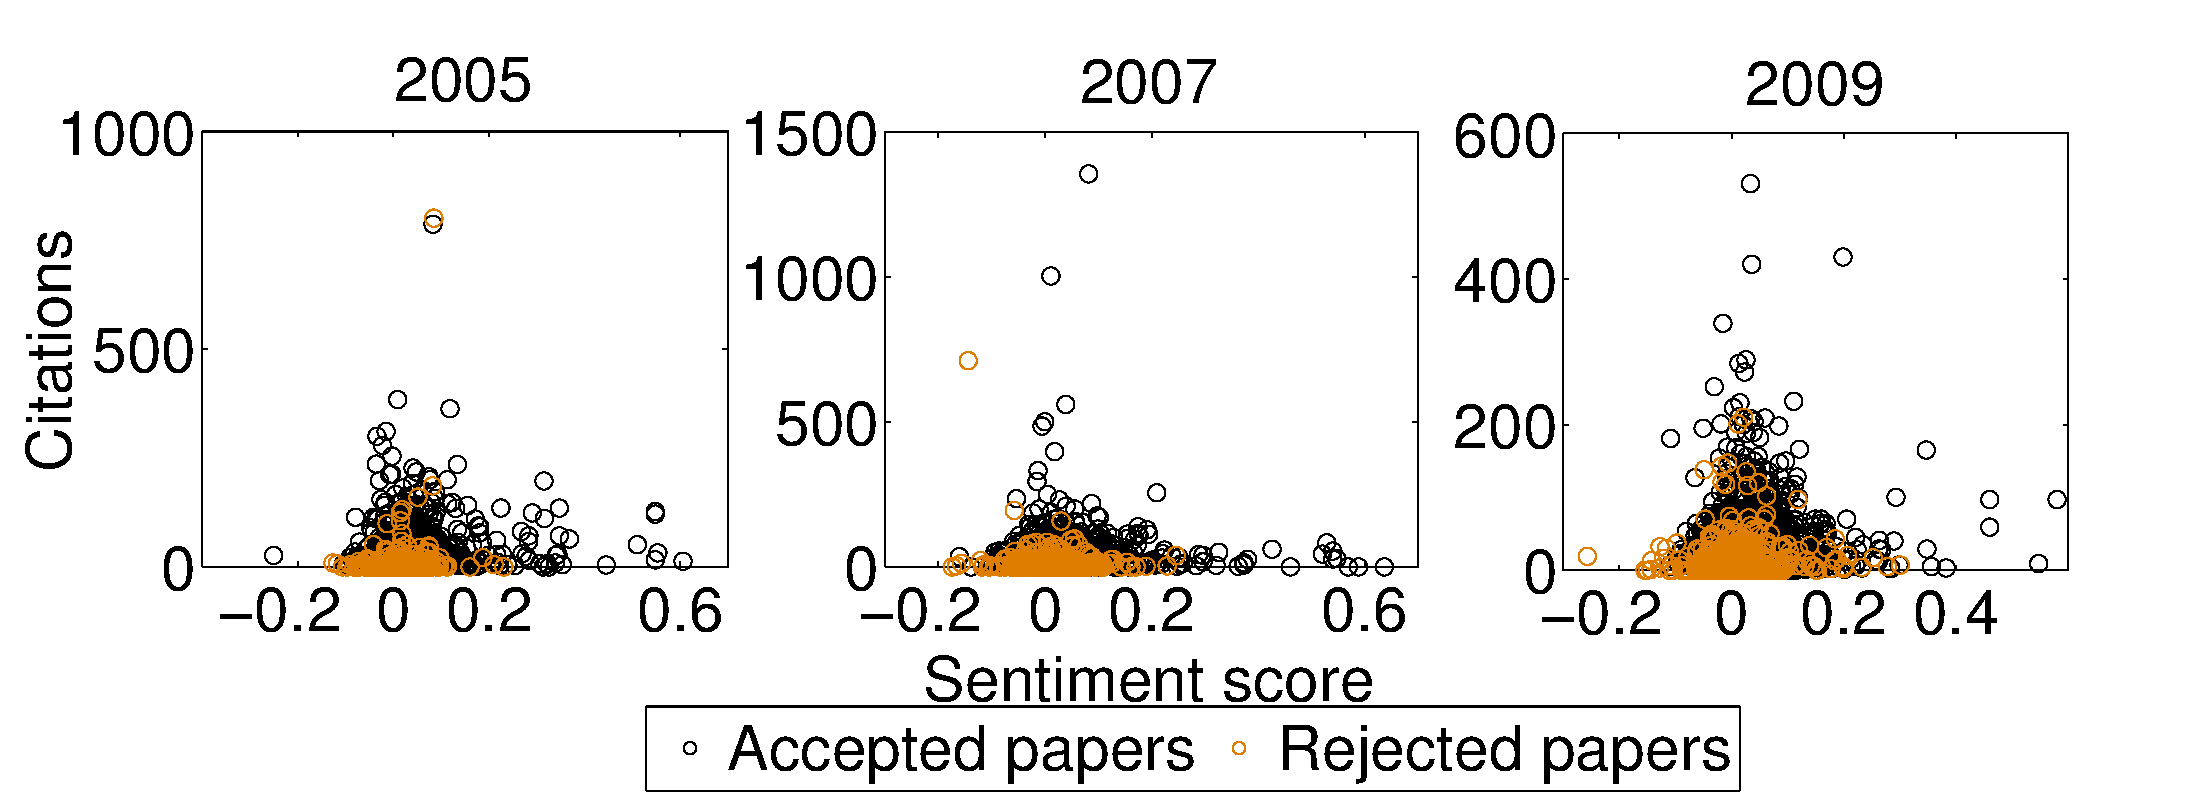
\includegraphics[scale=0.23]{./texfiles/Chapter_4/jcdl/figures/year_sent_cit-eps-converted-to.pdf}
\caption{Sentiment score versus citations for both accepted and rejected papers for the years 2005, 2007 and 2009. We find similar trends for other years as well.}
\label{fig12}
\vspace{3mm}
\end{figure}

To determine whether the overall sentiment of the reviews of a paper is related to the number of citations received by it, we plot for each paper (both accepted and rejected) the number of citations it received against the  sentiment score of the first round of review in figure~\ref{fig12}. Note that we segregate the papers based on the year of the publication or the rejection. We observe that the highly cited papers mostly have reviews with neutral or positive sentiment. Accepted papers with positive reviews are, on average, found to receive $25.27$ citations while those with negative reviews are found to receive $13.56$ citations.
However, there are cases where the accepted paper received highly positive reviews but was not cited. Conversely, there are cases where the sentiment was neutral but the paper garnered a large number of citations. Shown below are two such examples -- {\bf Case 1:} year of publication: 2006, sentiment score: 0.0234 (almost neutral), citations: 5812; {\bf Case 2:} year of publication: 2008, sentiment score: 0.65 (highly positive), citations: 6.


\begin{table}
\centering
\caption{Mean values of percentages of various categories of words in review reports of high and low cited papers where the means differ significantly.\vspace{3mm}}
\label{tab3}
\begin{tabular}{|l|l|l|l|}
\hline
Category                    & Dimension                                                   & \begin{tabular}[c]{@{}l@{}}High cited\\ papers\end{tabular} & \begin{tabular}[c]{@{}l@{}}Low cited\\ papers\end{tabular} \\ \hline \hline
\multirow{2}{*}{Linguistic} & Future tense                                                & 1.17                                                          & 1.05                                                         \\ \cline{2-4} 
                            & Negation                                                    & 0.72                                                          & 0.84                                                         \\ \hline
\multirow{4}{*}{Cognitive}  & Insight                                                     & 3.52                                                          & 3.16                                                         \\ \cline{2-4} 
                            & Causation                                                   & 2.60                                                          & 2.38                                                         \\ \cline{2-4} 
                            & Inclusive                                                   & 3.70                                                          & 3.43                                                         \\ \cline{2-4} 
                            & Exclusive                                                   & 1.28                                                          & 1.52                                                         \\ \hline
Affective                   & \begin{tabular}[c]{@{}l@{}}Positive \\ emotion\end{tabular} & 2.84                                                          & 2.70                                                         \\ \hline
\end{tabular}
\vspace{2mm}
\end{table}

For the rejected papers we observe that those which received neutral reviews but were rejected, tend to garner higher citations later compared to the ones which received negative reviews. There are certain exceptions as well, two of which are -- {\bf Case 1:} year of rejection: 2010, sentiment score: 0.27 (positive), citations: 1; {\bf Case 2:} year of rejection: 2007, sentiment score: -0.14 (negative), citations: 711.
Manual investigation of the review text shows that the papers which are highly cited after rejection were mainly rejected for not being in the scope of JHEP and not because of flawed results. 

\subsubsection*{Linguistic quality indicators (LQI)}

Here we check whether there are linguistic quality features present in the review reports which can serve as an indicator of the future impact of the paper. To our aim we use the LIWC\footnote{\url{http://liwc.wpengine.com/}} (Linguistic Inquiry and Word Count) text analysis tool~\cite{pennebaker2007development}. The tool provides, as output, percentage of words in different categories for an input text. The categories are broadly divided into linguistic (21 dimensions like pronouns, articles etc.), psychological (41 dimensions like affect, cognition etc.), personal concern (6 dimensions), informal language markers and punctuation apart from some general features like word count, words per sentence etc. We apply the LIWC tool on the review reports for our analysis and mainly focus on the linguistic and the psychological categories.
Next we check whether the LIWC features discussed earlier can also serve as indicators differentiating high and low cited papers. We rank the papers based on the number of citations they have received and consider the top 10\% as highly cited and the bottom 10\% as low cited papers. Note that we only consider the papers that were published before 2012 so that the papers have at least three years of citation history. In table~\ref{tab3} we report the mean percentage of words in different LIWC categories across all the papers (both high and low cited). We find several quality indicators here as well. The key observations are: (i) future tense is used more significantly in case of review reports of highly cited papers compared to low cited papers. On manually investigating the reviews of some of the highly cited papers we observe that statements like ``its result will become a useful addition to ..'' are prevalent; (ii) insightful and inclusive words are also used to a greater extent in review reports of highly cited papers compared to low cited papers; (iii) positive words are also more prevalent in highly cited papers as well.\\
Thus, these indicators show that the reviewers were, in many cases, indeed able to guess the quality of the paper as is evident from the review reports.



